% Options for packages loaded elsewhere
\PassOptionsToPackage{unicode}{hyperref}
\PassOptionsToPackage{hyphens}{url}
\PassOptionsToPackage{dvipsnames,svgnames,x11names}{xcolor}
%
\documentclass[
  letterpaper,
  authoryear]{elsarticle}

\usepackage{amsmath,amssymb}
\usepackage{iftex}
\ifPDFTeX
  \usepackage[T1]{fontenc}
  \usepackage[utf8]{inputenc}
  \usepackage{textcomp} % provide euro and other symbols
\else % if luatex or xetex
  \usepackage{unicode-math}
  \defaultfontfeatures{Scale=MatchLowercase}
  \defaultfontfeatures[\rmfamily]{Ligatures=TeX,Scale=1}
\fi
\usepackage{lmodern}
\ifPDFTeX\else  
    % xetex/luatex font selection
\fi
% Use upquote if available, for straight quotes in verbatim environments
\IfFileExists{upquote.sty}{\usepackage{upquote}}{}
\IfFileExists{microtype.sty}{% use microtype if available
  \usepackage[]{microtype}
  \UseMicrotypeSet[protrusion]{basicmath} % disable protrusion for tt fonts
}{}
\makeatletter
\@ifundefined{KOMAClassName}{% if non-KOMA class
  \IfFileExists{parskip.sty}{%
    \usepackage{parskip}
  }{% else
    \setlength{\parindent}{0pt}
    \setlength{\parskip}{6pt plus 2pt minus 1pt}}
}{% if KOMA class
  \KOMAoptions{parskip=half}}
\makeatother
\usepackage{xcolor}
\setlength{\emergencystretch}{3em} % prevent overfull lines
\setcounter{secnumdepth}{5}
% Make \paragraph and \subparagraph free-standing
\ifx\paragraph\undefined\else
  \let\oldparagraph\paragraph
  \renewcommand{\paragraph}[1]{\oldparagraph{#1}\mbox{}}
\fi
\ifx\subparagraph\undefined\else
  \let\oldsubparagraph\subparagraph
  \renewcommand{\subparagraph}[1]{\oldsubparagraph{#1}\mbox{}}
\fi


\providecommand{\tightlist}{%
  \setlength{\itemsep}{0pt}\setlength{\parskip}{0pt}}\usepackage{longtable,booktabs,array}
\usepackage{calc} % for calculating minipage widths
% Correct order of tables after \paragraph or \subparagraph
\usepackage{etoolbox}
\makeatletter
\patchcmd\longtable{\par}{\if@noskipsec\mbox{}\fi\par}{}{}
\makeatother
% Allow footnotes in longtable head/foot
\IfFileExists{footnotehyper.sty}{\usepackage{footnotehyper}}{\usepackage{footnote}}
\makesavenoteenv{longtable}
\usepackage{graphicx}
\makeatletter
\def\maxwidth{\ifdim\Gin@nat@width>\linewidth\linewidth\else\Gin@nat@width\fi}
\def\maxheight{\ifdim\Gin@nat@height>\textheight\textheight\else\Gin@nat@height\fi}
\makeatother
% Scale images if necessary, so that they will not overflow the page
% margins by default, and it is still possible to overwrite the defaults
% using explicit options in \includegraphics[width, height, ...]{}
\setkeys{Gin}{width=\maxwidth,height=\maxheight,keepaspectratio}
% Set default figure placement to htbp
\makeatletter
\def\fps@figure{htbp}
\makeatother

% These are extra latex packages that the document depends on
% 
\usepackage{siunitx}
\usepackage{booktabs}
\usepackage{longtable}
\usepackage{array}
\usepackage{multirow}
\usepackage{wrapfig}
\usepackage{float}
\usepackage{colortbl}
\usepackage{pdflscape}
\usepackage{tabu}
\usepackage{threeparttable}
\usepackage{threeparttablex}
\usepackage[normalem]{ulem}
\usepackage{makecell}
\usepackage{xcolor}
\makeatletter
\@ifpackageloaded{bookmark}{}{\usepackage{bookmark}}
\makeatother
\makeatletter
\@ifpackageloaded{caption}{}{\usepackage{caption}}
\AtBeginDocument{%
\ifdefined\contentsname
  \renewcommand*\contentsname{Table of contents}
\else
  \newcommand\contentsname{Table of contents}
\fi
\ifdefined\listfigurename
  \renewcommand*\listfigurename{List of Figures}
\else
  \newcommand\listfigurename{List of Figures}
\fi
\ifdefined\listtablename
  \renewcommand*\listtablename{List of Tables}
\else
  \newcommand\listtablename{List of Tables}
\fi
\ifdefined\figurename
  \renewcommand*\figurename{Figure}
\else
  \newcommand\figurename{Figure}
\fi
\ifdefined\tablename
  \renewcommand*\tablename{Table}
\else
  \newcommand\tablename{Table}
\fi
}
\@ifpackageloaded{float}{}{\usepackage{float}}
\floatstyle{ruled}
\@ifundefined{c@chapter}{\newfloat{codelisting}{h}{lop}}{\newfloat{codelisting}{h}{lop}[chapter]}
\floatname{codelisting}{Listing}
\newcommand*\listoflistings{\listof{codelisting}{List of Listings}}
\makeatother
\makeatletter
\makeatother
\makeatletter
\@ifpackageloaded{caption}{}{\usepackage{caption}}
\@ifpackageloaded{subcaption}{}{\usepackage{subcaption}}
\makeatother
\journal{Transportation Research Part A}
\ifLuaTeX
  \usepackage{selnolig}  % disable illegal ligatures
\fi
\usepackage[]{natbib}
\bibliographystyle{elsarticle-harv}
\usepackage{bookmark}

\IfFileExists{xurl.sty}{\usepackage{xurl}}{} % add URL line breaks if available
\urlstyle{same} % disable monospaced font for URLs
\hypersetup{
  pdftitle={Evaluating the effectiveness of an Incident Management Team expansion in Utah},
  pdfauthor={Joel Hyer; Grant Schultz; Gregory S. Macfarlane; Dennis Eggett},
  colorlinks=true,
  linkcolor={blue},
  filecolor={Maroon},
  citecolor={Blue},
  urlcolor={Blue},
  pdfcreator={LaTeX via pandoc}}

\setlength{\parindent}{6pt}
\begin{document}

\begin{frontmatter}
\title{Evaluating the effectiveness of an Incident Management Team
expansion in Utah}
\author[1]{Joel Hyer%
%
}

\author[1]{Grant Schultz%
%
}

\author[1]{Gregory S. Macfarlane%
%
}
 \ead{gregmacfarlane@gmail.com} 
\author[2]{Dennis Eggett%
%
}


\affiliation[1]{organization={Civil and Construction Engineering
Department, Brigham Young University},addressline={430
EB},city={Provo},postcode={84602},postcodesep={}}
\affiliation[2]{organization={Statistics Department, Brigham Young
University},city={Provo},postcode={84602},postcodesep={}}

\cortext[cor1]{Corresponding author}




        
\begin{abstract}
The abstract is a crucial component of any scientific paper, as it
provides a summary of the research and its main findings. This paper
provides guidelines for writing an effective scientific abstract. The
first step is to identify the key elements of the research, such as the
research question, methods, results, and conclusions. Next, the abstract
should be written in a clear and concise manner, using simple language
and avoiding technical jargon. The abstract should also be structured,
with a clear introduction, methods section, results section, and
conclusion. Additionally, the abstract should accurately and succinctly
convey the main findings of the research, highlighting the significance
and implications of the work. By following these guidelines, researchers
can ensure that their abstract effectively communicates the key aspects
of their research and attracts the attention of potential readers. -
Written by ChatGPT
\end{abstract}





\end{frontmatter}
    
\bookmarksetup{startatroot}

\section*{Preface}\label{preface}
\addcontentsline{toc}{section}{Preface}

\markboth{Preface}{Preface}

This is a template repository that I and my students can use to start
projects that will implement the workflow presented in my
\href{https://gregmacfarlane.github.io/lab/workflow.html}{lab
documentation}. It also serves as an instruction manual in this
workflow, a template article, and a sandbox for me to practice and
learn. I encourage students to use the
\href{https://quarto.org/docs/guide/}{Quarto Guide} as their primary
reference.

The document in this template renders to two\footnote{I hope to make it
  possible to render the article to a BYU Engineering thesis as well.
  Give me a bit of time.} outputs:

\begin{itemize}
\item
  A website
\item
  An Elsevier journal article
\end{itemize}

To render this document, use the command \texttt{quarto\ render} in your
terminal pointed at the working directory. This will create a website
available locally in a \texttt{\_book} folder and a PDF of the article
stored in that folder.

To render your website \emph{and} push its content to a live website,
use the command \texttt{quarto\ publish\ gh-pages}. Details of this
process are available on the
\href{https://quarto.org/docs/publishing/github-pages.html\#publish-command}{Quarto
guide}.

You can change the article to a different publisher by following the
directions at the \href{https://github.com/quarto-journals}{Quarto
Journal Templates GitHub} repository.

\bookmarksetup{startatroot}

\section{Introduction}\label{introduction}

The purpose of this report is to present the findings of the regression
analysis for the expansion of the Utah Department of Transportation
(UDOT) Incident Management Team (IMT) program and to determine the
effect of pertinent variables of crash data on IMT performance and user
impacts. In 2019, the Utah Department of Transportation (UDOT) funded a
research study to evaluate the effectiveness of an expanded Incident
Management Team (IMT) program. The number of IMTs patrolling Utah
roadways increased from 13 to 25 between 2018 and 2020. Crash data were
collected from the Utah Highway Patrol's (UHP) Computer-Aided Dispatch
(CAD) database and from the UDOT TransSuite database for 2018 and 2020.
Data were collected to compare IMT performance measures and the user
impacts of crashes responded to by IMTs for both years to evaluate the
benefits of the expanded IMT program. However, these data were
compromised due to the effects of the COVID-19 pandemic.

Because of the artificially low traffic volumes experienced during the
COVID-19 pandemic, one of the recommendations from the research was to
collect data in a future year without the impacts of COVID-19. The
research presented in this report collected data for 2022 using the same
methodology as the previous research to compare IMT performance measures
and user impacts of crashes in 2022 with those of 2018 after traffic
volumes had returned to a similar level as those of pre-pandemic levels.
The performance measures collected include IMT Response Time (RT),
Roadway Clearance Time (RCT), and IMT Incident Clearance Time (ICT). The
study also included performance measures of UHP RT and UHP ICT for UHP
units but focused primarily on IMT performance measures. The user
impacts quantified include the affected volume (AV) of vehicles, excess
travel time (ETT) -- or the total delay experienced by all roadway users
in a crash, and excess user cost (EUC) -- or the time cost of the delay
experienced by all roadway users.

Previous studies on traffic incident management have explored the
effectiveness of intelligent transportation systems (ITS) in responding
to crashes, the positive effect of IMT program policies on performance,
available data sources used to obtain and quantify IMT performance
measures, and the development of simulation models based on incident
probability to optimize the location of IMTs. However, a study has not
been to conducted to precisely quantify the user impacts of actual
incidents responded to by IMTs using in-field crash data and to
understand the correlations between specific user impacts and IMT
performance measures. Relating crash variables using in-field crash data
allows the benefits of IMTs to be more fully understood as well as guide
the allocation of resources to allow highway agencies to decrease the
delay and improve the safety experienced by roadway users.

This manuscript presents a comparison of IMT performance measures and
the user impacts of crashes responded to by IMTs for before the program
expansion (2018) and after the program expansion (2022). The sections
included are a literature review of previous related studies, the
methods used to obtain and clean crash data, the results of the
regression analysis, and the conclusions of the results.

\bookmarksetup{startatroot}

\section{Literature Review}\label{literature-review}

The literature review is not simply a ``review'' or a list of what has
been done in the past. This needs to a thoughtful synthesis that
accomplishes two things:

\begin{itemize}
\tightlist
\item
  Shows that you understand the previous efforts that other people have
  made on this problem.
\item
  Identifies the limitation or the gap in those previous efforts.
\end{itemize}

You will have already mentioned this gap in the introduction, but here
you need to build a solid case for why what you are doing is a
meaningful contribution.

Literature reviews do not have a specific guidelines for length or
number of citations. It's more about making a rhetorical argument; if
it's a new problem then the review can be shorter. But you'll need to
refer to previous attempts at the problem, the methods you are trying,
and other things.

\subsection{Citations and
Bibliographies}\label{citations-and-bibliographies}

Quarto has a robust method for generating citations. If you follow the
\href{https://quarto.org/docs/visual-editor/technical.html\#citations-from-zotero}{setup
instructions}, then you can easily search your database from inside
Rstudio after typing the \texttt{@} command. Keep your Zotero database
up-to-date and correct (and share it with your coauthors!) to minimize
the pain you will feel in writing articles.

Note that there are two ways to make citations. Doing \texttt{@key} will
give you a text citation, allowing you to refer to the author
mid-sentence.

\begin{quote}
\citet{ben-akivaDiscreteChoiceAnalysis1985} is the canonical reference
in choice modeling for transportation.
\end{quote}

But if you put the citation in brackets like \texttt{{[}@citationkey{]}}
you can make parenthetical citations. You can also give page numbers for
quotes or specific findings this way.

\begin{quote}
The difference in the choice model logsum can be used as a measure of
consumer surplus, and therefore accessibility improvement
\citep[p.~301]{ben-akivaDiscreteChoiceAnalysis1985}.
\end{quote}

\bookmarksetup{startatroot}

\section{Methodology}\label{methodology}

To estimate the impact of Utah's IMT program expansion, we collect data
from UDOT and UHP and model the impacts with a linear regression
analysis.

\subsection{Data}\label{data}

Describe the UHP incident database.

Describe the UDOT incident database.

Describe efforts to clean and filter the data for usable records.

\begin{table}

\caption{\label{tbl-severity}Descriptive Statistics of Data by Crash
Severity}

\centering{

\centering\centering
\begin{tabular}[t]{llrrrrrr}
\toprule
\multicolumn{2}{c}{ } & \multicolumn{2}{c}{Personal Injury (N=217)} & \multicolumn{2}{c}{Property Damage (N=180)} & \multicolumn{2}{c}{Fatal (N=6)} \\
\cmidrule(l{3pt}r{3pt}){3-4} \cmidrule(l{3pt}r{3pt}){5-6} \cmidrule(l{3pt}r{3pt}){7-8}
  &    & Mean & Std. Dev. & Mean & Std. Dev. & Mean & Std. Dev.\\
\midrule
IMT responding &  & 1.5 & 0.7 & 1.4 & 0.7 & 2.2 & 1.0\\
UHP responding &  & 3.5 & 1.7 & 2.9 & 1.4 & 10.5 & 3.7\\
Response time &  & 14.5 & 9.4 & 14.8 & 10.2 & 34.9 & 30.5\\
Roadway clearance time &  & 50.0 & 31.6 & 37.0 & 30.9 & 198.2 & 33.8\\
Incident clearance time &  & 65.5 & 35.3 & 59.7 & 28.7 & 190.5 & 8.9\\
Total lanes on roadway &  & 5.1 & 1.3 & 5.2 & 1.1 & 5.3 & 0.5\\
Lanes closed for incident &  & 2.0 & 1.1 & 1.9 & 0.9 & 4.2 & 1.6\\
Affected volume &  & 6978.7 & 5035.0 & 7218.5 & 4878.6 & 7029.2 & 4739.6\\
Excess travel time &  & 655.5 & 1052.8 & 572.5 & 876.5 & 1608.0 & 2832.2\\
\midrule\\
 &  & N & Pct. & N & Pct. & N & Pct.\\
Year & 2018 & 78 & 35.9 & 90 & 50.0 & 2 & 33.3\\
 & 2022 & 139 & 64.1 & 90 & 50.0 & 4 & 66.7\\
Period & Afternoon Off Peak & 87 & 40.1 & 62 & 34.4 & 3 & 50.0\\
 & AM Peak & 42 & 19.4 & 46 & 25.6 & 0 & 0.0\\
 & Morning Off Peak & 1 & 0.5 & 1 & 0.6 & 2 & 33.3\\
 & Night Off Peak & 21 & 9.7 & 4 & 2.2 & 1 & 16.7\\
 & PM Peak & 66 & 30.4 & 67 & 37.2 & 0 & 0.0\\
\bottomrule
\end{tabular}

}

\end{table}%

Table~\ref{tbl-severity} presents descriptive statistics of the cleaned
incident data by crash severity. Virtually all of the records are either
property damage or personal injury crashes (approximately half each),
with a handful of fatal crashes. The mean excess travel time for these
fatal crashes is approximately three times higher than for the other
more common crash types, though the wide standard errors and the high
degree of skewness make conclusive statements about this question
somewhat difficult.

\begin{figure}

\centering{

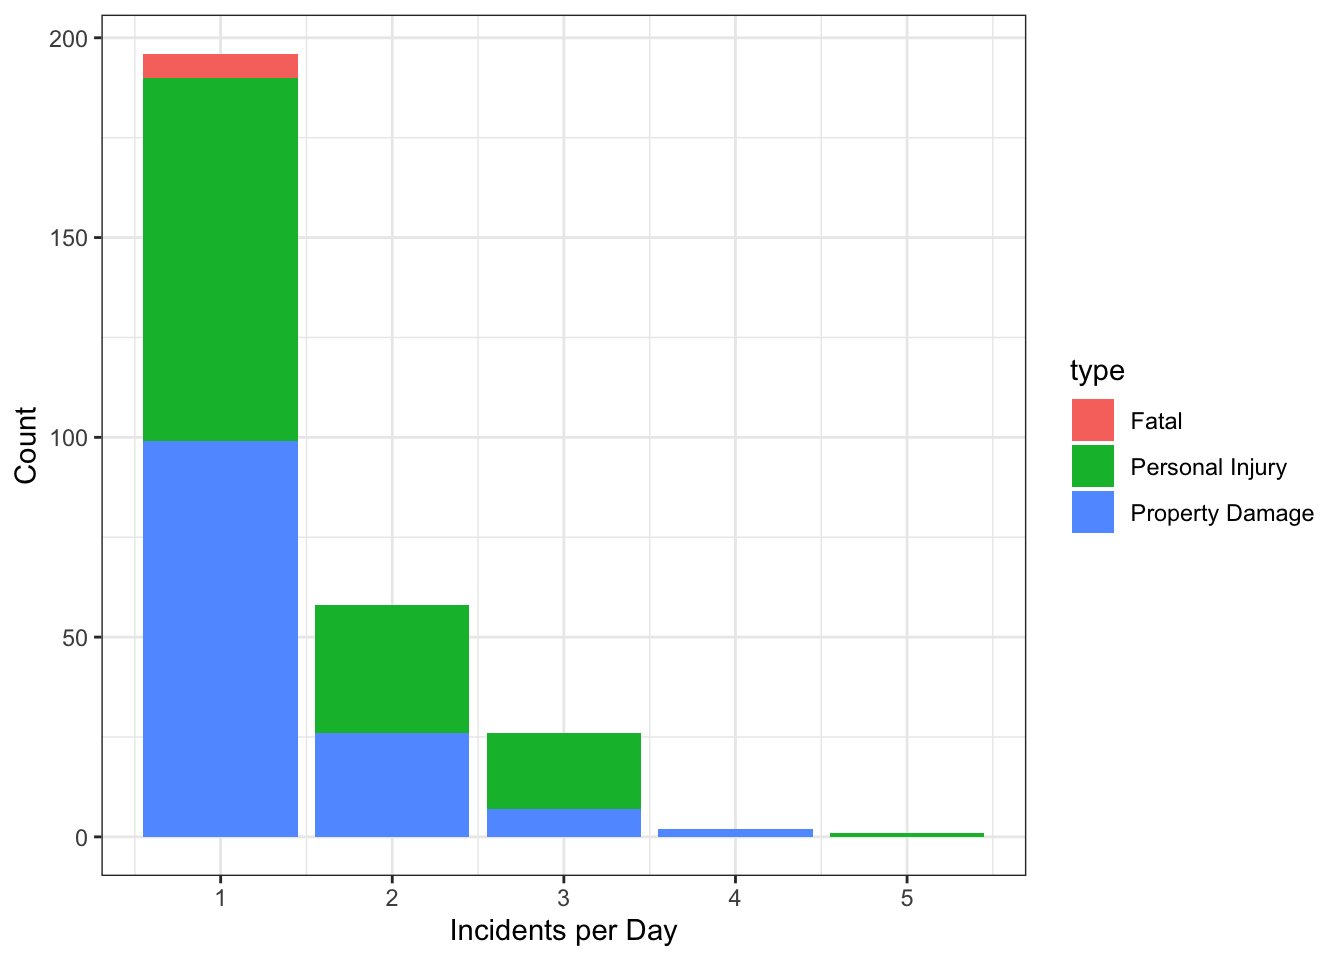
\includegraphics{03_methods_files/figure-pdf/fig-frequency-1.pdf}

}

\caption{\label{fig-frequency}IMT-responding incidents per day by crash
severity.}

\end{figure}%

Figure~\ref{fig-frequency} shows a distribution of incidents by day.
This might not be the most relevant plot, but it's the one that I put
together.

\subsection{Models}\label{models}

We hypothesize that the increase in IMT units decreased response time as
well as decreased excess travel time. This suggests two models, \[ 
\log(\mathrm{IMT\ Response\ Time}_i) = X_i\beta
\] and \[ 
\log(\mathrm{Excess\ Travel\ Time}_i) = X_i\beta + \delta\log(\mathrm{IMT\ Response\ Time}_i)
\] where the index \(i\) denotes a single incident, \(X\) is a vector of
controlling variables --- the number of responding units, the size of
the roadways, etc. --- and \(\beta\) are estimated coefficients.

\bookmarksetup{startatroot}

\section{Results}\label{results}

\begin{table}

\caption{\label{tbl-rtmodels}Estimated Models of IMT Response Time}

\centering{

\centering
\begin{tabular}[t]{lcc}
\toprule
  & Base & Year\\
\midrule
(Intercept) & 2.943*** & 3.034***\\
 & (0.266) & (0.270)\\
Fatal crash (ref. property damage) & 0.892+ & 0.879+\\
 & (0.460) & (0.459)\\
Total lanes on roadway & -0.057 & -0.053\\
 & (0.042) & (0.042)\\
N. IMT units & -0.139+ & -0.141+\\
 & (0.074) & (0.074)\\
N. UHP units & -0.006 & -0.004\\
 & (0.031) & (0.031)\\
2022 dummy (ref. 2018) &  & -0.179+\\
 &  & (0.103)\\
\midrule
Num.Obs. & 384 & 384\\
R2 & 0.025 & 0.032\\
R2 Adj. & 0.012 & 0.017\\
\bottomrule
\multicolumn{3}{l}{\rule{0pt}{1em}+ p $<$ 0.1, * p $<$ 0.05, ** p $<$ 0.01, *** p $<$ 0.001}\\
\multicolumn{3}{l}{\rule{0pt}{1em}Dependent variable: $textbackslash{}log$(Response time).}\\
\multicolumn{3}{l}{\rule{0pt}{1em}Standard errors in parentheses}\\
\end{tabular}

}

\end{table}%

Table~\ref{tbl-rtmodels} shows regression estimates of models predicting
the natural log of the IMT response time. A Base model

\begin{table}

\caption{\label{tbl-ettmodels}Estimated Models of Excess Travel Time}

\centering{

\centering
\begin{tabular}[t]{lccc}
\toprule
  & Base & Year & Year and RT\\
\midrule
(Intercept) & 3.649*** & 4.088*** & 3.553***\\
 & (0.423) & (0.422) & (0.570)\\
Fatal crash (ref. property damage) & -0.551 & -0.530 & -0.658\\
 & (0.712) & (0.694) & (0.704)\\
Total lanes on roadway & 0.182* & 0.198** & 0.174*\\
 & (0.072) & (0.070) & (0.072)\\
N. IMT units & 0.523*** & 0.519*** & 0.545***\\
 & (0.123) & (0.119) & (0.124)\\
2022 dummy (ref. 2018) &  & -0.807*** & -0.354\\
 &  & (0.170) & (0.470)\\
IMT response time &  &  & 0.249+\\
 &  &  & (0.137)\\
2022 \$\textbackslash{}times\$ IMT Response time &  &  & -0.173\\
 &  &  & (0.178)\\
\midrule
Num.Obs. & 403 & 403 & 384\\
R2 & 0.061 & 0.112 & 0.115\\
R2 Adj. & 0.052 & 0.100 & 0.099\\
\bottomrule
\multicolumn{4}{l}{\rule{0pt}{1em}+ p $<$ 0.1, * p $<$ 0.05, ** p $<$ 0.01, *** p $<$ 0.001}\\
\multicolumn{4}{l}{\rule{0pt}{1em}Dependent variable: $textbackslash{}log$(Excess  travel time).}\\
\multicolumn{4}{l}{\rule{0pt}{1em}Standard errors in parentheses}\\
\end{tabular}

}

\end{table}%

Table~\ref{tbl-ettmodels} shows estimates of regression models
predicting the excess travel time.

\subsubsection{Predictions}\label{predictions}

\bookmarksetup{startatroot}

\section{Conclusions}\label{conclusions}

This section need not be overly long. You should address any limitations
of your results, such as dependence on underlying assumptions or
geographic scope. You should also provide a map for future research.

Finally, you should underline the contributions of this work and any
practical relevance.

\bookmarksetup{startatroot}

\section*{References}\label{references}
\addcontentsline{toc}{section}{References}

\markboth{References}{References}

\renewcommand{\bibsection}{}
\bibliography{references.bib,IMTRegression.bib}




\end{document}
